\documentclass[a4paper,11pt]{article}
\usepackage{graphicx}
\usepackage[numbers]{natbib}
% Used https://tex.stackexchange.com/questions/420588/numbered-citations-in-latex for citation numbes
\usepackage{array}
\usepackage{booktabs}
\usepackage{longtable}

\begin{document}
Appendix

\section{Glossary}
\begin{itemize}
	\item Bagging – using sampling with replacement from the data to create artificial training data (bootstrap samples)
	\item Bayesian Optimisation – a function used to run through an array of different hyperparameters for a machine learning model
	\item BFGS - (Broyden-Fletcher-Goldfarb-Shanno quasi-Newton algorithm) a second order derivative used to help optimise linear regression.\citep{brownlee_gentle_2021} (paraphrased)
	\item Decision Tree Regression – splits the data into distinct regions with the region’s mean being the response to a prediction \citep{james_gareth_introduction_2021} (paraphrased)
	\item Hyperparameter – a parameter of the machine learning model (so named as machine learning models are used to find the parameters of a model)
	\item Lasso Regression – Least Absolute Shrinkage and Selection Operator. Tries to eliminate as many features as possible when performing the regression to have as sparse a model as possible \citep{stephanie_lasso_2015}
	\item Linear Regression: an algorithm which attempts to fit an equation of the form $Y = wX + c$ to the data so that its error to the true value is minimised as far as possible
	\item Normalised: the data is shifted so that its mean is zero and rescaled to move its standard deviation to 1. I am excluding the zero/one categorical columns from this, as it doesn’t make sense to include them.
	\item Random Forest Regression – a collection of decision tree regressors (hence the forest) that behaves as a single model as the average prediction is returned from the collection of decision tree results. Each individual tree is trained using “bagging and random features” \citep{schapire_robert_random_2001}. A random subset of features is given to each tree.
	\item Ridge Regression – allows for models where the number of features is greater than the number of predictors and allows interactions between features. “Adds just enough bias to make the estimates reasonably reliable” \citep{stephanie_ridge_2017} (paraphrased and directly quoted) 
\end{itemize}

\section{Intermediate results}
\begin{longtable}{m{3.5cm}m{6.5cm}m{1.5cm}m{1.5cm}m{1.5cm}}
\toprule
Type & Hyper-Parameters & RMSE & MAE & Accuracy (1-NMSE) \\
\midrule
Linear Regression & Default (columns: model, year, mileage, fuel type, MPG, engine size) & 4782.14 & 3602.55 & -0.04 \\
\addlinespace
Linear Regression & Default (columns: model, year, mileage, fuel type, MPG, engine size), Normalised & 2427.54 & 1717.89 & 0.73 \\
\addlinespace
Linear Regression & Lambda', 0.0002972, 'Learner', 'leastsquares', 'Regularization', 'ridge', 'Solver', 'bfgs' (columns: model, year, mileage, fuel type, MPG, engine size), Normalised & 1828.18 & 1346.7 & 0.85 \\
\addlinespace
Linear Regression & Lambda', 0.0002972, 'Learner', 'leastsquares', 'Regularization', 'ridge', 'Solver', 'bfgs' (columns: model, year, mileage, fuel type, MPG, engine size), Normalised, with validation data & 1837.15 & 1350.96 & 0.85 \\
\addlinespace
Linear Regression & Lambda', 0.000010015, 'Learner', 'leastsquares', 'Regularization', 'ridge', 'Solver', 'bfgs' (columns: model, year, mileage, fuel type, MPG, engine size), Normalised, validation & 1859.48 & 1358.33 & 0.84 \\
\addlinespace
Linear Regression & Lambda', 0.000010015, 'Learner', 'leastsquares', 'Regularization', 'ridge', 'Solver', 'bfgs' (columns: model, year, mileage, fuel type, MPG, engine size), Normalised & 1826.26 & 1347.21 & 0.85 \\
\addlinespace
Linear Regression & Lambda', 0.000010015, 'Learner', 'leastsquares', 'Regularization', 'ridge', 'Solver', 'bfgs', 'Kfold', 5 (columns: model, year, mileage, fuel type, MPG, engine size), Normalised (1st model) & 1818.02 & 1344.83 & 0.85 \\
\addlinespace
Random Forest & Default (columns: model, year, mileage, fuel type, MPG, engine size) & 1279.66 & 889.33 & 0.93 \\
\addlinespace
Random Forest (technically boosted forest) & MinLeafSize, 31, Method, LSBoost, NumLearningCycles, 193, LearnRate 0.38119. (columns: model, year, mileage, fuel type, MPG, engine size). & 1185.69 & 837.56 & 0.94 \\
\addlinespace
Random Forest & MinLeafSize, 31, Method, Bag, NumLearningCycles, 193, (columns: model, year, mileage, fuel type, MPG, engine size). & 1398.75 & 968.24 & 0.91 \\
\addlinespace
Random Forest & MinLeafSize, 1, Method, Bag, NumLearningCycles, 499, (columns: model, year, mileage, fuel type, MPG, engine size). & 1175.02 & 838.02 & 0.94 \\
\addlinespace
Random Forest & MinLeafSize, 1, Method, Bag, NumLearningCycles, 450, (columns: model, year, mileage, fuel type, MPG, engine size). & 1175.03 & 838.63 & 0.94 \\
\addlinespace
Random Forest & MinLeafSize, 1, Method, Bag, NumLearningCycles, 50, (columns: model, year, mileage, fuel type, MPG, engine size). & 1178.42 & 839.35 & 0.94 \\
\addlinespace
Random Forest & MinLeafSize, 1, Method, Bag, NumLearningCycles, 500, (columns: model, year, mileage, fuel type, MPG, engine size). & 1174.68 & 838.28 & 0.94 \\
\addlinespace
Random Forest & MinLeafSize, 1, Method, Bag, NumLearningCycles, 499, (columns: model, year, mileage, fuel type, MPG, engine size). & 1177.4 & 839.2 & 0.94 \\
\addlinespace
\bottomrule
\end{longtable}

\begin{figure}[!htb] % trick from https://tex.stackexchange.com/questions/32598/force-latex-image-to-appear-in-the-section-in-which-its-declared
\centering
% using https://tex.stackexchange.com/questions/198386/input-figures-from-sub-folders
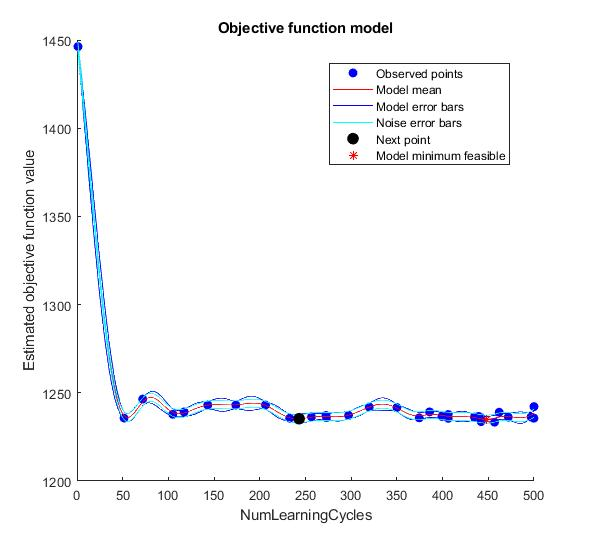
\includegraphics[height=7.38cm]{img/RFNumLearCyclesVMinMRSE}
\caption{RF Number of Learners versus RMSE}
\end{figure}

From the below graph you can see that there is not much difference between using 50 trees and 500. I have kept it at 499 as the results against the test set were better (if we cared about computational efficiency, we might cap at around 50 trees).
Using K-Fold validation on Random Forest made the results worse.

\section{Implementation Details}

\section{References}
\bibliographystyle{plainnat}
\bibliography{MyLibrary}

\end{document}